% Options for packages loaded elsewhere
\PassOptionsToPackage{unicode}{hyperref}
\PassOptionsToPackage{hyphens}{url}
\PassOptionsToPackage{dvipsnames,svgnames,x11names}{xcolor}
%
\documentclass[
  11pt,
]{article}
\usepackage{amsmath,amssymb}
\usepackage{iftex}
\ifPDFTeX
  \usepackage[T1]{fontenc}
  \usepackage[utf8]{inputenc}
  \usepackage{textcomp} % provide euro and other symbols
\else % if luatex or xetex
  \usepackage{unicode-math} % this also loads fontspec
  \defaultfontfeatures{Scale=MatchLowercase}
  \defaultfontfeatures[\rmfamily]{Ligatures=TeX,Scale=1}
\fi
\usepackage{lmodern}
\ifPDFTeX\else
  % xetex/luatex font selection
  \setmainfont[]{Latin Modern Roman}
  \setsansfont[]{Latin Modern Sans}
  \setmonofont[]{DejaVu Sans Mono}
\fi
% Use upquote if available, for straight quotes in verbatim environments
\IfFileExists{upquote.sty}{\usepackage{upquote}}{}
\IfFileExists{microtype.sty}{% use microtype if available
  \usepackage[]{microtype}
  \UseMicrotypeSet[protrusion]{basicmath} % disable protrusion for tt fonts
}{}
\makeatletter
\@ifundefined{KOMAClassName}{% if non-KOMA class
  \IfFileExists{parskip.sty}{%
    \usepackage{parskip}
  }{% else
    \setlength{\parindent}{0pt}
    \setlength{\parskip}{6pt plus 2pt minus 1pt}}
}{% if KOMA class
  \KOMAoptions{parskip=half}}
\makeatother
\usepackage{xcolor}
\usepackage[margin=25mm]{geometry}
\usepackage{color}
\usepackage{fancyvrb}
\newcommand{\VerbBar}{|}
\newcommand{\VERB}{\Verb[commandchars=\\\{\}]}
\DefineVerbatimEnvironment{Highlighting}{Verbatim}{commandchars=\\\{\}}
% Add ',fontsize=\small' for more characters per line
\newenvironment{Shaded}{}{}
\newcommand{\AlertTok}[1]{\textcolor[rgb]{1.00,0.00,0.00}{\textbf{#1}}}
\newcommand{\AnnotationTok}[1]{\textcolor[rgb]{0.38,0.63,0.69}{\textbf{\textit{#1}}}}
\newcommand{\AttributeTok}[1]{\textcolor[rgb]{0.49,0.56,0.16}{#1}}
\newcommand{\BaseNTok}[1]{\textcolor[rgb]{0.25,0.63,0.44}{#1}}
\newcommand{\BuiltInTok}[1]{\textcolor[rgb]{0.00,0.50,0.00}{#1}}
\newcommand{\CharTok}[1]{\textcolor[rgb]{0.25,0.44,0.63}{#1}}
\newcommand{\CommentTok}[1]{\textcolor[rgb]{0.38,0.63,0.69}{\textit{#1}}}
\newcommand{\CommentVarTok}[1]{\textcolor[rgb]{0.38,0.63,0.69}{\textbf{\textit{#1}}}}
\newcommand{\ConstantTok}[1]{\textcolor[rgb]{0.53,0.00,0.00}{#1}}
\newcommand{\ControlFlowTok}[1]{\textcolor[rgb]{0.00,0.44,0.13}{\textbf{#1}}}
\newcommand{\DataTypeTok}[1]{\textcolor[rgb]{0.56,0.13,0.00}{#1}}
\newcommand{\DecValTok}[1]{\textcolor[rgb]{0.25,0.63,0.44}{#1}}
\newcommand{\DocumentationTok}[1]{\textcolor[rgb]{0.73,0.13,0.13}{\textit{#1}}}
\newcommand{\ErrorTok}[1]{\textcolor[rgb]{1.00,0.00,0.00}{\textbf{#1}}}
\newcommand{\ExtensionTok}[1]{#1}
\newcommand{\FloatTok}[1]{\textcolor[rgb]{0.25,0.63,0.44}{#1}}
\newcommand{\FunctionTok}[1]{\textcolor[rgb]{0.02,0.16,0.49}{#1}}
\newcommand{\ImportTok}[1]{\textcolor[rgb]{0.00,0.50,0.00}{\textbf{#1}}}
\newcommand{\InformationTok}[1]{\textcolor[rgb]{0.38,0.63,0.69}{\textbf{\textit{#1}}}}
\newcommand{\KeywordTok}[1]{\textcolor[rgb]{0.00,0.44,0.13}{\textbf{#1}}}
\newcommand{\NormalTok}[1]{#1}
\newcommand{\OperatorTok}[1]{\textcolor[rgb]{0.40,0.40,0.40}{#1}}
\newcommand{\OtherTok}[1]{\textcolor[rgb]{0.00,0.44,0.13}{#1}}
\newcommand{\PreprocessorTok}[1]{\textcolor[rgb]{0.74,0.48,0.00}{#1}}
\newcommand{\RegionMarkerTok}[1]{#1}
\newcommand{\SpecialCharTok}[1]{\textcolor[rgb]{0.25,0.44,0.63}{#1}}
\newcommand{\SpecialStringTok}[1]{\textcolor[rgb]{0.73,0.40,0.53}{#1}}
\newcommand{\StringTok}[1]{\textcolor[rgb]{0.25,0.44,0.63}{#1}}
\newcommand{\VariableTok}[1]{\textcolor[rgb]{0.10,0.09,0.49}{#1}}
\newcommand{\VerbatimStringTok}[1]{\textcolor[rgb]{0.25,0.44,0.63}{#1}}
\newcommand{\WarningTok}[1]{\textcolor[rgb]{0.38,0.63,0.69}{\textbf{\textit{#1}}}}
\usepackage{longtable,booktabs,array}
\usepackage{calc} % for calculating minipage widths
% Correct order of tables after \paragraph or \subparagraph
\usepackage{etoolbox}
\makeatletter
\patchcmd\longtable{\par}{\if@noskipsec\mbox{}\fi\par}{}{}
\makeatother
% Allow footnotes in longtable head/foot
\IfFileExists{footnotehyper.sty}{\usepackage{footnotehyper}}{\usepackage{footnote}}
\makesavenoteenv{longtable}
\usepackage{graphicx}
\makeatletter
\def\maxwidth{\ifdim\Gin@nat@width>\linewidth\linewidth\else\Gin@nat@width\fi}
\def\maxheight{\ifdim\Gin@nat@height>\textheight\textheight\else\Gin@nat@height\fi}
\makeatother
% Scale images if necessary, so that they will not overflow the page
% margins by default, and it is still possible to overwrite the defaults
% using explicit options in \includegraphics[width, height, ...]{}
\setkeys{Gin}{width=\maxwidth,height=\maxheight,keepaspectratio}
% Set default figure placement to htbp
\makeatletter
\def\fps@figure{htbp}
\makeatother
\setlength{\emergencystretch}{3em} % prevent overfull lines
\providecommand{\tightlist}{%
  \setlength{\itemsep}{0pt}\setlength{\parskip}{0pt}}
\setcounter{secnumdepth}{5}
% definitions for citeproc citations
\NewDocumentCommand\citeproctext{}{}
\NewDocumentCommand\citeproc{mm}{%
  \begingroup\def\citeproctext{#2}\cite{#1}\endgroup}
\makeatletter
 % allow citations to break across lines
 \let\@cite@ofmt\@firstofone
 % avoid brackets around text for \cite:
 \def\@biblabel#1{}
 \def\@cite#1#2{{#1\if@tempswa , #2\fi}}
\makeatother
\newlength{\cslhangindent}
\setlength{\cslhangindent}{1.5em}
\newlength{\csllabelwidth}
\setlength{\csllabelwidth}{3em}
\newenvironment{CSLReferences}[2] % #1 hanging-indent, #2 entry-spacing
 {\begin{list}{}{%
  \setlength{\itemindent}{0pt}
  \setlength{\leftmargin}{0pt}
  \setlength{\parsep}{0pt}
  % turn on hanging indent if param 1 is 1
  \ifodd #1
   \setlength{\leftmargin}{\cslhangindent}
   \setlength{\itemindent}{-1\cslhangindent}
  \fi
  % set entry spacing
  \setlength{\itemsep}{#2\baselineskip}}}
 {\end{list}}
\usepackage{calc}
\newcommand{\CSLBlock}[1]{\hfill\break\parbox[t]{\linewidth}{\strut\ignorespaces#1\strut}}
\newcommand{\CSLLeftMargin}[1]{\parbox[t]{\csllabelwidth}{\strut#1\strut}}
\newcommand{\CSLRightInline}[1]{\parbox[t]{\linewidth - \csllabelwidth}{\strut#1\strut}}
\newcommand{\CSLIndent}[1]{\hspace{\cslhangindent}#1}
\ifLuaTeX
\usepackage[bidi=basic]{babel}
\else
\usepackage[bidi=default]{babel}
\fi
\babelprovide[main,import]{american}
\ifPDFTeX
\else
\babelfont{rm}[]{Latin Modern Roman}
\fi
% get rid of language-specific shorthands (see #6817):
\let\LanguageShortHands\languageshorthands
\def\languageshorthands#1{}
\usepackage{fancyhdr}
\usepackage{microtype}
\usepackage{needspace}
\usepackage{float}
\floatplacement{figure}{H}
\usepackage{caption}
\usepackage{seqsplit}
\captionsetup{font=small,labelfont=bf}
\pagestyle{fancy}
\fancyhf{}
\fancyhead[L]{\footnotesize\textsc{Wind Tunnel · TACITUS}}
\fancyhead[R]{\footnotesize Working paper WT-2026-01 · v1.1}
\fancyfoot[C]{\small\thepage}
\setlength{\headheight}{14pt}
\setlength{\emergencystretch}{3em}
\setlength{\parskip}{5pt}
\setlength{\parindent}{0pt}
\AtBeginEnvironment{CSLReferences}{\interlinepenalty=10000}
\renewcommand{\headrulewidth}{0.3pt}
\AtBeginDocument{\hypersetup{pdftitle={Wind Tunnel: Evidence-Separated Population Modeling for AI-Assisted Research Preparation},pdfauthor={TACITUS},pdfsubject={Working paper WT-2026-01, version 1.1; not independently peer-reviewed},pdfkeywords={population modeling, questionnaire preparation, provenance, language models}}}
\let\originalsection\section
\renewcommand{\section}{\Needspace{5\baselineskip}\originalsection}
\ifLuaTeX
  \usepackage{selnolig}  % disable illegal ligatures
\fi
\usepackage{bookmark}
\IfFileExists{xurl.sty}{\usepackage{xurl}}{} % add URL line breaks if available
\urlstyle{same}
\hypersetup{
  pdftitle={Wind Tunnel: Evidence-Separated Population Modeling for AI-Assisted Research Preparation},
  pdfauthor={TACITUS},
  pdflang={en-US},
  colorlinks=true,
  linkcolor={teal},
  filecolor={Maroon},
  citecolor={Blue},
  urlcolor={teal},
  pdfcreator={LaTeX via pandoc}}

\title{Wind Tunnel: Evidence-Separated Population Modeling for
AI-Assisted Research Preparation}
\author{TACITUS}
\date{24 November 2026}

\begin{document}
\maketitle
\begin{abstract}
AI-generated responses can help researchers articulate assumptions and
prepare questions, but agreement with a demographic frame does not
establish agreement with human attitudes. Wind Tunnel is an experimental
workspace that keeps demographic inputs, human survey evidence, authored
hypotheses, and generated outputs separately identifiable. This report
documents its released US questionnaire-preparation recipe and a
retrospective aggregate comparison. The recipe prompts a language model
across twelve age-by-education cells and combines the resulting answer
distributions using fitted 2020--2024 American Community Survey
household-adult masses. Authored qualitative dossiers enter a separate
wording review with zero population weight. Against twelve 2024 General
Social Survey institutional-confidence distributions, mean total
variation is 2.48 percentage points for a 2022 human-survey persistence
baseline, 7.50 for a national model call, and 8.16 for the conditioned,
weighted recipe. The conditioned recipe has no lower mean error in this
fixed comparison. The contrast changes prompting and call structure as
well as weighting, and does not identify a causal effect of weighting
alone. Frozen study revisions make inputs and assumptions inspectable;
the public package permits exact score replay. We specify an intended
workflow for questionnaire preparation, followed by expert and
human-participant checks, and the prospective tests required to assess
its value. The contribution is a documented research procedure and an
openly inspectable negative comparison, not validated measurement of
public opinion.
\end{abstract}

\textbf{Working paper WT-2026-01 · Version 1.1.} Published by TACITUS.
Independent peer review has not been completed. This revision clarifies
interpretation and research use; the benchmark data and generation run
are unchanged. Correspondence:
\href{mailto:hello@tacitus.me}{\nolinkurl{hello@tacitus.me}}.

\textbf{Keywords:} computational social science; questionnaire
preparation; synthetic survey responses; population modeling;
provenance; language models.

\section{Introduction}\label{introduction}

Research preparation involves more than drafting plausible questions. An
analyst needs to define the people and period of interest, make a
proposal's trade-offs explicit, distinguish observations from
assumptions, and decide which interpretations require a check with
people. A generative model can assist with that preparation. Its fluent
answer, however, is not a measurement of the population named in its
prompt.

Wind Tunnel is an experimental workspace for organizing audience
definitions, questionnaire versions, model-assisted exploration, and
human evidence. Its central design choice is to retain the evidentiary
role of each record. A demographic count is different from an attitude
estimate; an authored dossier is different from a respondent; a
generated answer distribution is different from completed fieldwork.
Saved study revisions carry these distinctions into subsequent review
and reports.

This report makes three contributions. It specifies the released US
cell-based generation and aggregation procedure; it describes the
records needed to inspect and revisit an analysis; and it releases an
aggregate benchmark whose scores can be independently recomputed. The
empirical question is whether this particular conditioned recipe agrees
more closely with a fixed human-survey reference than a national model
call. On the selected battery, it does not. The result is useful for
directing further work even though it does not validate a broad
predictive product.

The paper concerns the source revision and run recorded in Appendix B.
It evaluates an answer-distribution recipe, not the causal effect of
questionnaire wording or the usefulness of every interface feature. The
intended next application is research preparation with explicit human
validation, rather than substituting generated responses for a
representative survey.

\section{Related work and methodological
position}\label{related-work-and-methodological-position}

Language-model simulation has reproduced some patterns in particular
human datasets (\citeproc{ref-argyle2023}{Argyle et al. 2023}), while
other evaluations identify errors in subgroup relationships and
sensitivity to prompts and models (\citeproc{ref-bisbee2024}{Bisbee et
al. 2024}). A model's response to a wording perturbation can also differ
from a human response to that perturbation
(\citeproc{ref-tjuatja2024}{Tjuatja et al. 2024}). These findings
motivate separate evaluation of distributional agreement,
questionnaire-review usefulness, and generalization to a new population
or period.

Demographic fitting and response estimation serve different functions.
Adjusting a table to known margins is a statistical construction
(\citeproc{ref-deming1940}{Deming and Stephan 1940}). Multilevel
regression and poststratification additionally fits a response model and
aggregates its predictions over population cells
(\citeproc{ref-gelman1997}{Gelman and Little 1997}). Wind Tunnel's
released numeric recipe aggregates model-supplied distributions with
demographic masses. It does not fit a multilevel model to human answers,
so its demographic weighting is not evidence of calibrated MRP or valid
public-opinion measurement.

The reporting approach draws on model cards
(\citeproc{ref-mitchell2019}{Mitchell et al. 2019}), structured
simulation documentation (\citeproc{ref-grimm2020}{Grimm et al. 2020}),
and survey disclosure standards (\citeproc{ref-aapor}{American
Association for Public Opinion Research n.d.}). PROV-O offers a
conceptual vocabulary for records, transformations, and responsibility
(\citeproc{ref-prov2013}{Lebo, Sahoo, and McGuinness 2013}). These
references inform the design; they do not certify its estimates or
establish full implementation of their standards. In this system,
provenance makes a result easier to question and reproduce at a declared
level.

\section{Evidence, universe, and target
quantity}\label{evidence-universe-and-target-quantity}

\subsection{Evidentiary roles}\label{evidentiary-roles}

Table 1 distinguishes what the principal records can support. Keeping
these roles explicit prevents an appealing model character or a
generated answer from silently becoming an observation about people.

\begin{longtable}[]{@{}
  >{\raggedright\arraybackslash}p{(\columnwidth - 4\tabcolsep) * \real{0.3333}}
  >{\raggedright\arraybackslash}p{(\columnwidth - 4\tabcolsep) * \real{0.3333}}
  >{\raggedright\arraybackslash}p{(\columnwidth - 4\tabcolsep) * \real{0.3333}}@{}}
\caption{Evidentiary roles are distinct from a ranking of document
quality. A source can be accurately preserved while an interpretation of
it remains mistaken.}\tabularnewline
\toprule\noalign{}
\begin{minipage}[b]{\linewidth}\raggedright
Record
\end{minipage} & \begin{minipage}[b]{\linewidth}\raggedright
Example
\end{minipage} & \begin{minipage}[b]{\linewidth}\raggedright
Interpretation
\end{minipage} \\
\midrule\noalign{}
\endfirsthead
\toprule\noalign{}
\begin{minipage}[b]{\linewidth}\raggedright
Record
\end{minipage} & \begin{minipage}[b]{\linewidth}\raggedright
Example
\end{minipage} & \begin{minipage}[b]{\linewidth}\raggedright
Interpretation
\end{minipage} \\
\midrule\noalign{}
\endhead
\bottomrule\noalign{}
\endlastfoot
Source estimate & Published ACS table & A dated estimate under its
source universe and definitions \\
Derived quantity & Adult age-band count & A documented transformation of
source cells \\
Fitted representation & Age-by-education population masses & A
construction compatible with declared controls and donor assumptions \\
Human evidence & Weighted GSS answer distribution & A survey estimate
under that instrument and design \\
Statistical response estimate & A separately fitted human-response model
& Inference conditional on the fitted model and its validation \\
Authored hypothesis & Qualitative dossier or scenario override & An
analyst's assumption for investigation \\
Generated output & Model-supplied cell answer shares & The output of the
specified computational procedure \\
\end{longtable}

\subsection{Population foundation and
estimand}\label{population-foundation-and-estimand}

The US demographic artifact uses 2020--2024 ACS five-year tables and
Public Use Microdata Sample documentation (\citeproc{ref-acs2024}{U.S.
Census Bureau 2026}). It retains source periods, geography, variable
definitions, and relevant universes. A five-year period estimate is not
a contemporaneous census count, and overlapping geographic products
cannot simply be added.

The numeric recipe uses four adult age groups---18--34, 35--44, 45--64,
and at least 65---and three education groups: high school or less; some
college or an associate degree; and a bachelor's degree or higher. Their
cross-product contains twelve cells. The artifact retains resident-adult
and household-adult masses. The benchmark selects the latter to better
align its declared universe with the GSS household-adult study
population. Broad universe alignment does not remove differences in
coverage, language, survey mode, nonresponse, or field dates.

For question \(q\) and substantive answer category \(k\), the scientific
target would be the proportion of the eligible population giving answer
\(k\) under a specified instrument and field period. The released
benchmark observes a weighted survey estimate of that quantity, denoted
\(y_{qk}\), rather than population truth. Comparison with \(y_{qk}\)
measures agreement with this survey reference. A general claim about
population attitudes would additionally require the appropriate
survey-design uncertainty and external-validity argument.

The age-by-education masses come from the fitted artifact, rather than
an assumption that age and education are independent. Compatibility with
demographic controls is evidence about this construction; it does not
measure institutional confidence or recover every unobserved local joint
distribution. A demographic label or added personality description
supplies no independent observation of a person's political beliefs.

\subsection{Human evidence and qualitative
dossiers}\label{human-evidence-and-qualitative-dossiers}

Human evidence retains an exact item, substantive coding, eligible
population, field period, weights, and available design information.
Different instruments cannot be treated as interchangeable merely
because they address related civic topics. Item-specific answered counts
and weighted denominators remain relevant when questions have different
forms or missing answers.

The US catalog also includes six authored qualitative dossiers, of which
up to two can enter a study's wording-review stage. A dossier describes
hypothesized constraints, priorities, protected values, trade-offs,
information context, a counterexample, and a fieldwork probe.
Protected-values research motivates one aspect of this description
(\citeproc{ref-baron1997}{Baron and Spranca 1997}). A dossier's
population weight is zero. Its role is to prompt investigation of an
assumption, not to establish a measured personality type or allocate
public opinion to a demographic group.

\section{Released computational
procedure}\label{released-computational-procedure}

\subsection{Frozen study revision}\label{frozen-study-revision}

A study revision binds the proposal versions, questionnaire, audience
selection, cell masses, selected dossiers, and execution recipe. It
records source and fitted-artifact hashes, the runtime hash, requested
model, temperature, thinking setting, and output cap. The result retains
actual execution information and the count of human interviews. The
generated US pretest reports zero human interviews.

Figure 1 separates the numeric and qualitative paths. Demographic masses
determine aggregation weights; the model supplies answer shares.
Dossiers enter a separate review. A saved revision makes it possible to
locate which assumptions accompanied a finding, including after an
analyst changes an input or a colleague continues the work.

\begin{figure}
\centering
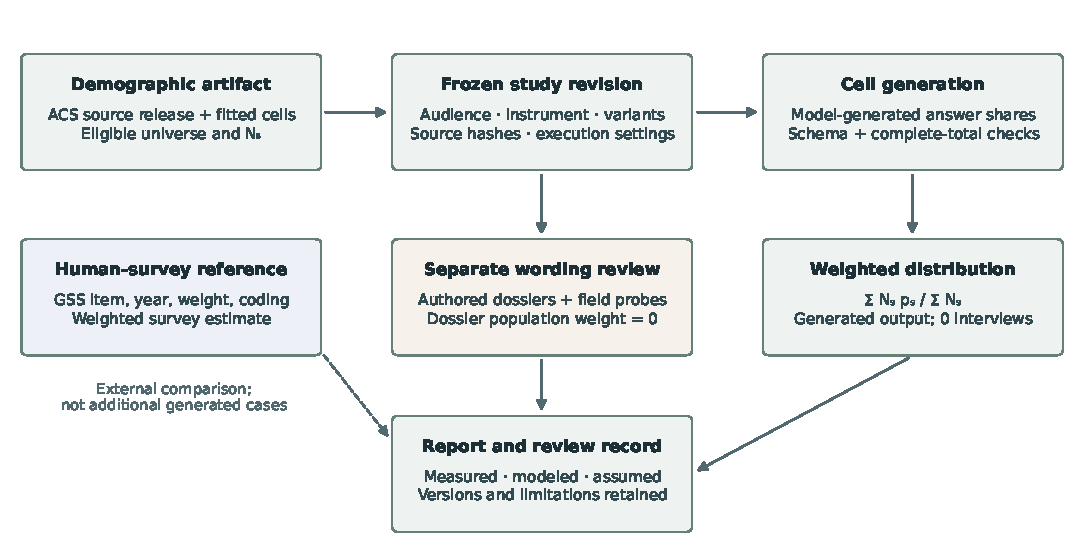
\includegraphics[width=0.98\textwidth,height=\textheight]{figures/evidence-flow.pdf}
\caption{Computational and evidentiary roles in the released US recipe.
Solid arrows show dependencies. Human-survey evidence provides an
external comparison; authored dossiers inform a separate wording review
with zero population weight. The provenance record connects inputs and
outputs without validating the model-supplied response probabilities.}
\end{figure}

\subsection{Generation, validation, and
aggregation}\label{generation-validation-and-aggregation}

For each proposal version, the model receives the same required
multiple-choice questionnaire for every included demographic cell. This
recipe accepts one to four questions, each with two to eight distinct
options. Its contract excludes randomized presentation, conditional
branching, and an additional don't-know option. Each output gives
integer percentages in the instrument's option order, summing to 100 per
question. Invalid or incomplete responses fail the structural check.

Let \(s\) index included cells, \(q\) a question, \(k\) a category,
\(N_s\) the chosen fitted population mass, and \(p_{sqk}\) a validated
model share on the unit interval. Aggregation produces

\[
\widehat{p}_{qk}=\frac{\sum_{s\in S}N_s p_{sqk}}{\sum_{s\in S}N_s}.
\]

This operation is deterministic given the cell masses and model outputs.
Its weights control contributions; they do not establish that
\(p_{sqk}\) estimates the corresponding human response probability. The
twelve cell calls are not twelve independent respondents, and large
population masses do not create a large generated survey sample.

A separate structured model review receives the proposal, questionnaire,
and selected dossiers and returns possible wording issues and field
checks using supplied identifiers. Dossiers are excluded from numeric
aggregation. Differences between proposal versions are differences under
the chosen model recipe. They can suggest a question to investigate, but
do not identify a causal wording effect in people.

\subsection{Provenance and reproducibility
boundary}\label{provenance-and-reproducibility-boundary}

The small graph relevant to this workflow connects source release,
demographic artifact, audience, instrument, proposal version, execution,
finding, and report. ``Derived from,'' ``used in,'' and ``compared
with'' have different meanings. A new source or assumption creates
another revision rather than rewriting the old receipt.

This is conceptually related to a context capsule: evidence,
instructions, assumptions, and versions travel with a work product. It
is not a claim that the private Wind Tunnel implementation implements
the generic TACITUS App capsule interchange or a complete ontology
reasoner. A graph can preserve an incorrect assumption as faithfully as
a sound one.

Three reproducibility levels should be separated. \textbf{Score replay}
recomputes metrics from released distributions. \textbf{Input
reconstruction} also requires exact source extracts, transformations,
cell masses, questionnaire, and prompts. \textbf{Generation replay}
further depends on provider availability and stochastic execution. The
public package establishes score replay. Hashes identify records; they
cannot recover unavailable inputs or guarantee the same hosted-model
response. Full independent reconstruction of the private generation
pipeline remains outside this release.

\section{Retrospective GSS
comparison}\label{retrospective-gss-comparison}

\subsection{Design and comparators}\label{design-and-comparators}

The public benchmark uses twelve recurring institutional-confidence
items in the 2022 and 2024 GSS cross-sections
(\citeproc{ref-gss2026}{NORC at the University of Chicago 2026}). It
retains substantive response codes 1--3 and applies \texttt{WTSSNRPS}
within each year's eligible, answered item set. The releases have 3,544
and 3,309 eligible cases respectively; item-specific answered counts and
weighted denominators remain in the aggregate data. The split-wording
labor-union item, \texttt{CONLABOR}, is excluded.

The 2024 weighted distribution is the reference. Three inputs are scored
against it: the corresponding 2022 human distribution, one national
model call per item, and the twelve-cell conditioned and weighted
recipe. The earlier human survey is a \textbf{temporal-persistence
baseline} on recurring questions, not a contemporaneous human experiment
against the model. The receipt identifies \texttt{gemini-3.5-flash-lite}
on Vertex AI, completed on 23 November 2026. It identifies this run
rather than whichever model the product later offers.

The national and cell-based recipes use the substantive item text and
2024 context. Their contrast changes demographic prompting, call
structure, and aggregation together. It therefore tests the released
recipe as a whole; it cannot isolate a causal effect of demographic
weighting alone. The comparison also does not estimate the incremental
value of the separate dossier review.

The design is retrospective: the target answers were public before
generation and training exposure is possible. The run's hashes are not
evidence of target concealment or prospective preregistration. Survey
forms, presentation, mode, language, and field dates can differ across
the human waves. Matching the recurring item and substantive codes does
not establish equivalence in every other respect.

\subsection{Metrics}\label{metrics}

For an input distribution \(p\) and the weighted reference \(y\) over
three categories, total variation is

\[
\operatorname{TV}(p,y)=\frac{1}{2}\sum_{k=1}^{3}|p_k-y_k|.
\]

The report expresses \(100\operatorname{TV}\) in percentage points: the
answer mass that must move to match the reference. This is a
distributional discrepancy, not a model's probability of being wrong.

The released scorer also computes half-scaled multiclass Brier loss
averaged over reference category shares:

\[
\operatorname{B}(p,y)=\frac{1}{2}\left(1+\sum_{k=1}^{3}p_k^2-2\sum_{k=1}^{3}p_k y_k\right).
\]

This is the expected proper squared-error loss against a one-hot
category drawn with shares \(y\) (\citeproc{ref-brier1950}{Brier 1950}).
Even \(p=y\) gives nonzero loss when the reference has multiple
categories. The excess over this reference-matched loss is
\(\frac{1}{2}\sum_k(p_k-y_k)^2\). Thus absolute Brier values reflect
category uncertainty as well as disagreement; they should not be read as
aggregate squared distances or as calibration evidence for future
events. Both reported metrics are lower-is-better within this fixed
comparison.

\subsection{Results and
interpretation}\label{results-and-interpretation}

\begin{longtable}[]{@{}lrr@{}}
\caption{Equal-item means across twelve institutional-confidence
questions. Values are replayed from the unchanged aggregate release. TV
is in percentage points; Brier uses the half-scaled convention
above.}\tabularnewline
\toprule\noalign{}
Method & Mean TV (pp) & Mean Brier \\
\midrule\noalign{}
\endfirsthead
\toprule\noalign{}
Method & Mean TV (pp) & Mean Brier \\
\midrule\noalign{}
\endhead
\bottomrule\noalign{}
\endlastfoot
2022 human survey & 2.48 & 0.29274 \\
National model call & 7.50 & 0.29771 \\
Census-weighted model & 8.16 & 0.29892 \\
\end{longtable}

The temporal-persistence baseline has the lowest mean discrepancy on
both metrics for this battery. The conditioned recipe's mean TV is 0.66
percentage points above the national model call; its difference from the
earlier human baseline is 5.68 points. These results provide no mean
improvement for the conditioned recipe in the released comparison. They
do not show that weighting always harms generation, that earlier surveys
generally outperform models, or that the separate wording-review feature
is ineffective.

\begin{figure}
\centering
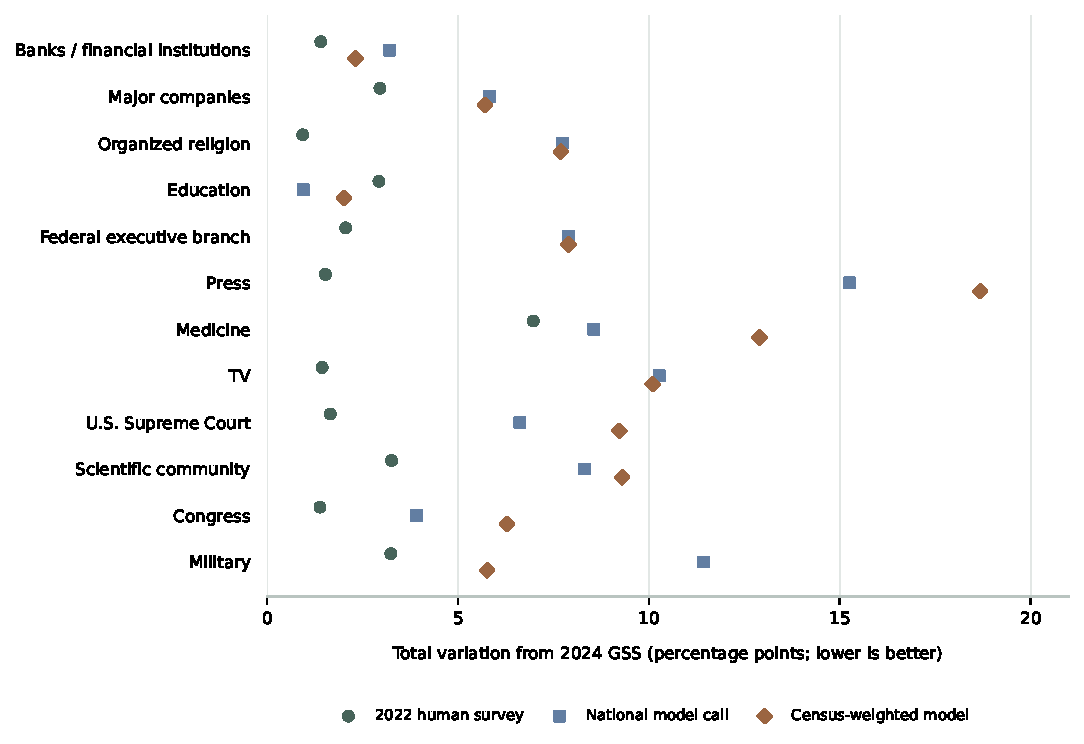
\includegraphics[width=0.98\textwidth,height=\textheight]{figures/benchmark-items.pdf}
\caption{Item-level total variation from weighted 2024 GSS estimates.
The unchanged release compares the two model recipes with the 2022
temporal-persistence baseline. These related items and one generation
run are descriptive evidence; the figure includes no inferential
uncertainty intervals.}
\end{figure}

The conditioned recipe's largest discrepancy is confidence in the press,
at 18.68 TV points. Individual items sometimes favor a model recipe even
though the overall mean favors the human baseline. Appendix A reports
all items. The twelve questions form a related, selected battery rather
than independent random draws from all possible research tasks; no
confidence interval or significance claim is attached to the mean
differences.

\section{Intended research use: prepare, inspect, then test with
people}\label{intended-research-use-prepare-inspect-then-test-with-people}

A useful next workflow starts with a research question and ends with a
check in the target setting. For example, a municipal researcher
considering a six-month extension of evening bus service might need to
describe an afternoon-frequency reduction that funds it. The
illustration below is an authored research-design example, not an
evaluated deployment or a measured claim about riders.

\begin{longtable}[]{@{}
  >{\raggedright\arraybackslash}p{(\columnwidth - 4\tabcolsep) * \real{0.3333}}
  >{\raggedright\arraybackslash}p{(\columnwidth - 4\tabcolsep) * \real{0.3333}}
  >{\raggedright\arraybackslash}p{(\columnwidth - 4\tabcolsep) * \real{0.3333}}@{}}
\caption{Illustrative research-preparation workflow. Generated
hypotheses may direct attention, while expert assessment and
human-participant evidence establish whether a revision works for the
intended study.}\tabularnewline
\toprule\noalign{}
\begin{minipage}[b]{\linewidth}\raggedright
Stage
\end{minipage} & \begin{minipage}[b]{\linewidth}\raggedright
Work product
\end{minipage} & \begin{minipage}[b]{\linewidth}\raggedright
Human decision or check
\end{minipage} \\
\midrule\noalign{}
\endfirsthead
\toprule\noalign{}
\begin{minipage}[b]{\linewidth}\raggedright
Stage
\end{minipage} & \begin{minipage}[b]{\linewidth}\raggedright
Work product
\end{minipage} & \begin{minipage}[b]{\linewidth}\raggedright
Human decision or check
\end{minipage} \\
\midrule\noalign{}
\endhead
\bottomrule\noalign{}
\endlastfoot
Define the study & Population, place, period, proposal wording, intended
decision & Confirm the universe and which trade-off respondents must
understand \\
Explore assumptions & Saved audience, explicit cell recipe, qualitative
probes & Inspect stereotypes, missing perspectives, and unsupported
assumptions \\
Review the instrument & Versioned question, possible ambiguity,
comparison wording & Assess whether costs, timing, alternatives, and
answer options are understood \\
Pilot and revise & Human interview or pilot evidence kept separately
from generated output & Test comprehension and measurement, then record
accepted revisions \\
\end{longtable}

In the bus example, a model might flag that ``improve service'' conceals
the funding trade-off or that ``evening'' lacks an operating-time
definition. A researcher would inspect those suggestions, preserve the
exact wording and why it changed, and test relevant versions through
expert review, cognitive interviews, or a human pilot. A finding that
people understand a question better must come from that subsequent
evaluation; it does not follow from a plausible model critique.

The value proposition to test is a reduction in avoidable
research-preparation work at an acceptable error rate. Useful outcomes
include important instrument defects found, false alarms, missed
defects, time to a usable revised questionnaire, and clarity of the
handover to another researcher. A synthetic answer-distribution score
alone does not establish any of these outcomes.

\section{Limitations and evaluation
agenda}\label{limitations-and-evaluation-agenda}

\subsection{Limits of the current
evidence}\label{limits-of-the-current-evidence}

The results concern a narrow institutional-confidence battery, one
recorded generation run, and a particular model--prompt--population
recipe. Public target data leave contamination unresolved. Repeated runs
and model-version changes are not characterized. Age and education may
omit relevant sources of heterogeneity, and conditioning can reinforce
stereotypes rather than recover within-cell disagreement.

The human references are survey estimates. Coverage, nonresponse,
wording, modes, weights, and periods affect comparability. Released
aggregates do not support a complete design-based variance analysis
without the appropriate source design information. Model variability and
survey-estimation uncertainty should be reported separately in a future
study, rather than combined into a synthetic ``margin of error.''

Score replay is public, but the exact private workbook mapping,
generation templates, and complete input construction are not
independently reconstructible from this package. Numeric agreement is
also separate from practical usefulness in questionnaire preparation.
These limitations define what the current study can support, rather than
supplying an argument against testing other uses.

\subsection{Prospective distributional
evaluation}\label{prospective-distributional-evaluation}

Before a stronger evaluation, freeze the population universe,
instrument, item-selection rule, data cutoff, model snapshot, prompts,
aggregation, and primary metrics. Register the analysis before
generating or exposing the target answers. Include a defensible
contemporaneous human reference with its design uncertainty, a simple
historical or marginal baseline, and an unconditioned model comparator.
Use new items and settings, with relevant subgroup and
insufficient-coverage cases.

A factorial or otherwise explicitly controlled ablation should separate
demographic prompting, aggregation weights, number of model calls, and
dossier review. Multiple runs and model snapshots should assess
stability. Report item and subgroup failures as well as overall errors.
This would permit a more specific conclusion about which component helps
under which conditions.

\subsection{Evaluation of questionnaire
preparation}\label{evaluation-of-questionnaire-preparation}

Run a separate blinded study of the practical workflow in Table 3.
Independent researchers should identify consequential instrument defects
before seeing the AI suggestions. Compare ordinary researcher
preparation with AI-assisted preparation under matched time or cost
accounting. Reviewers should score relevant defects, unsupported
criticisms, omissions, and the usefulness of proposed revisions,
retaining disagreements and failures.

Cognitive interviews or a human pilot can then test whether accepted
changes improve comprehension or the intended measurement. Record
preparation, model usage, reviewer effort, and revision time. These are
proposed experiments. The present benchmark establishes neither their
results nor a general analyst-time saving.

\section{Conclusion}\label{conclusion}

Wind Tunnel makes the inputs and assumptions of AI-assisted research
preparation inspectable. Its released US procedure combines explicit
demographic masses with model-supplied answer shares, keeps qualitative
dossiers separate from population weighting, and preserves the study
context in frozen records. On the selected GSS battery, the earlier
human-survey persistence baseline has lower mean error than both model
recipes, and the conditioned recipe has no mean advantage over the
national call. This is a bounded negative result, not a universal
ranking of human and machine research. The next scientific question is
whether the documented workflow helps researchers prepare better
instruments and investigate assumptions, as tested with independent
review and human evidence.

\section{Availability, authorship, and
disclosures}\label{availability-authorship-and-disclosures}

\textbf{Publication.} TACITUS. 2026. \emph{Wind Tunnel:
Evidence-Separated Population Modeling for AI-Assisted Research
Preparation.} Working paper WT-2026-01, version 1.1.
\href{https://github.com/sargonxg/TACITUS-Knowledge-Pipeline-open/tree/main/research/wind-tunnel-methodology/v1.1}{Versioned
source, figures, and reproducibility materials}.
\href{https://tacitus.me/research/wind-tunnel/paper/}{Version 1.0
archive}. Independent peer review has not been completed; no journal
acceptance, DOI registration, or external endorsement is claimed.

\textbf{Authorship and interests.} TACITUS develops and publishes the
software and has a commercial interest in it. AI assistance was used in
manuscript preparation and source/code checks. This assistance is not
independent scientific review. The paper separates replayed scores,
implementation descriptions, illustrations, and proposed evaluations.

\textbf{Materials and rights.} The public benchmark supplies aggregate
distributions, item identifiers, source references, run hashes, and a
scorer. It includes no individual GSS respondent records. GSS, ACS, and
cited instruments retain their source terms; original manuscript and
figures follow the repository's license. The private application and
generation templates are not represented as open source. Researchers
remain responsible for appropriate consent, privacy, source terms, and
communication of uncertainty.

\renewcommand{\thetable}{A\arabic{table}}
\setcounter{table}{0}

\section*{Appendix A. Item-level
comparison}\label{appendix-a.-item-level-comparison}
\addcontentsline{toc}{section}{Appendix A. Item-level comparison}

\begin{longtable}[]{@{}
  >{\raggedright\arraybackslash}p{(\columnwidth - 6\tabcolsep) * \real{0.2500}}
  >{\raggedleft\arraybackslash}p{(\columnwidth - 6\tabcolsep) * \real{0.2500}}
  >{\raggedleft\arraybackslash}p{(\columnwidth - 6\tabcolsep) * \real{0.2500}}
  >{\raggedleft\arraybackslash}p{(\columnwidth - 6\tabcolsep) * \real{0.2500}}@{}}
\caption{Total variation in percentage points by retained item. The
released aggregate file contains every three-category distribution. Each
item contributes equally to Table 2.}\tabularnewline
\toprule\noalign{}
\begin{minipage}[b]{\linewidth}\raggedright
GSS item / institution
\end{minipage} & \begin{minipage}[b]{\linewidth}\raggedleft
2022 human
\end{minipage} & \begin{minipage}[b]{\linewidth}\raggedleft
National model
\end{minipage} & \begin{minipage}[b]{\linewidth}\raggedleft
Weighted model
\end{minipage} \\
\midrule\noalign{}
\endfirsthead
\toprule\noalign{}
\begin{minipage}[b]{\linewidth}\raggedright
GSS item / institution
\end{minipage} & \begin{minipage}[b]{\linewidth}\raggedleft
2022 human
\end{minipage} & \begin{minipage}[b]{\linewidth}\raggedleft
National model
\end{minipage} & \begin{minipage}[b]{\linewidth}\raggedleft
Weighted model
\end{minipage} \\
\midrule\noalign{}
\endhead
\bottomrule\noalign{}
\endlastfoot
\texttt{confinan} · Banks and financial institutions & 1.40 & 3.20 &
2.31 \\
\texttt{conbus} · Major companies & 2.95 & 5.83 & 5.71 \\
\texttt{conclerg} · Organized religion & 0.93 & 7.74 & 7.70 \\
\texttt{coneduc} · Education & 2.93 & 0.95 & 2.02 \\
\texttt{confed} · Executive branch of the federal government & 2.06 &
7.89 & 7.89 \\
\texttt{conpress} · Press & 1.53 & 15.25 & 18.68 \\
\texttt{conmedic} · Medicine & 6.97 & 8.56 & 12.90 \\
\texttt{contv} · TV & 1.44 & 10.27 & 10.10 \\
\texttt{conjudge} · U.S. Supreme Court & 1.65 & 6.62 & 9.23 \\
\texttt{consci} · Scientific community & 3.26 & 8.32 & 9.30 \\
\texttt{conlegis} · Congress & 1.38 & 3.91 & 6.28 \\
\texttt{conarmy} · Military & 3.24 & 11.42 & 5.76 \\
\end{longtable}

\section*{Appendix B. Reproduction
record}\label{appendix-b.-reproduction-record}
\addcontentsline{toc}{section}{Appendix B. Reproduction record}

The benchmark and scorer are pinned to public commit
\texttt{\seqsplit{2b51dfee375b1ee0e5fd1ee7a99edd1623d8cac4}}, directory
\texttt{research/wind-tunnel-us/v1}. The application implementation
described is version 3.12.1 at commit
\texttt{\seqsplit{546b24d1f47671ff917ac1a09eb3bc5d9ab54d15}}. This
publication revision changes exposition, not the underlying input
distributions or generation run.

From the public repository root, score replay requires Node.js 20 or
later:

\begin{Shaded}
\begin{Highlighting}[]
\ExtensionTok{node}\NormalTok{ research/wind{-}tunnel{-}us/v1/score.mjs verify }\DataTypeTok{\textbackslash{}}
\NormalTok{  research/wind{-}tunnel{-}us/v1/benchmark.json}
\end{Highlighting}
\end{Shaded}

Rebuilding the paper additionally requires Python 3 with Matplotlib,
Pandoc with citeproc, and XeLaTeX. Run \texttt{build.py} and
\texttt{verify.py} in this publication directory. No inference call is
made. The manifest records the benchmark checksum and all publication
artifacts; a checksum identifies bytes rather than validating the
underlying scientific claim.

The existing receipt preserves protocol hash
\texttt{\seqsplit{f4752712c623d1fec445d913ebd50645df9620b2e6feb9f693b2d01eb14b941a}},
input hash
\texttt{\seqsplit{4beacae21cafa9bc39b9a87d4b29fafee3657f81ea1c15d63f270d1757b6a9f9}},
and output hash
\texttt{\seqsplit{7f1fbffe45f03aa2254710c816b0eb60f93780aca98b35ea2e544d2db6de6a04}}.
They identify the recorded run, not target concealment or end-to-end
independent replication.

\section*{Appendix C. Optional legacy scenario
model}\label{appendix-c.-optional-legacy-scenario-model}
\addcontentsline{toc}{section}{Appendix C. Optional legacy scenario
model}

The archived operational reference describes a deterministic Signal
engine with 27 authored behavioral archetypes, ten input signal
dimensions, and 34 operational indicators. The archetypes and
coefficients are modeling choices, separate from the source-backed
demographic artifact and the GSS comparison. Moral Foundations research
motivates some constructs (\citeproc{ref-atari2023}{Atari et al. 2023}),
but does not validate the engine's coefficients or establish its
archetypes as measured population groups.

Historical labels such as ``Backlash Probability'' describe model
scales, not calibrated event probabilities. Related indicators share
inputs and are not independent confirmations. The 13-event historical
showcase is a curated retrospective diagnostic and can be affected by
reuse during heuristic development. A seeded 50-run perturbation
ensemble explores declared assumptions; its output percentiles are not
human sampling errors or validated forecast intervals. Model
interpretation of canonical Signal outputs adds generated prose, not
another independent numeric estimate.

These legacy diagnostics support inspection of an exploratory model. The
GSS comparison does not validate them, and they should not be merged
with human evidence or the cell-based recipe merely because they appear
in the same research workspace.

\section*{References}\label{references}
\addcontentsline{toc}{section}{References}

\phantomsection\label{refs}
\begin{CSLReferences}{1}{0}
\bibitem[\citeproctext]{ref-aapor}
American Association for Public Opinion Research. n.d. {``Transparency
Initiative: Disclosure Standards.''} Accessed November 23, 2026.
\url{https://aapor.org/standards-and-ethics/transparency-initiative/}.

\bibitem[\citeproctext]{ref-argyle2023}
Argyle, Lisa P., Ethan C. Busby, Nancy Fulda, Joshua R. Gubler,
Christopher Rytting, and David Wingate. 2023. {``Out of One, Many: Using
Language Models to Simulate Human Samples.''} \emph{Political Analysis}
31 (3): 337--51. \url{https://doi.org/10.1017/pan.2023.2}.

\bibitem[\citeproctext]{ref-atari2023}
Atari, Mohammad, Jonathan Haidt, Jesse Graham, Sena Koleva, Sean T.
Stevens, and Morteza Dehghani. 2023. {``Morality Beyond the WEIRD: How
the Nomological Network of Morality Varies Across Cultures.''}
\emph{Journal of Personality and Social Psychology} 125 (5): 1157--88.
\url{https://doi.org/10.1037/pspp0000470}.

\bibitem[\citeproctext]{ref-baron1997}
Baron, Jonathan, and Mark Spranca. 1997. {``Protected Values.''}
\emph{Organizational Behavior and Human Decision Processes} 70 (1):
1--16. \url{https://doi.org/10.1006/obhd.1997.2690}.

\bibitem[\citeproctext]{ref-bisbee2024}
Bisbee, James, Joshua D. Clinton, Cassy Dorff, Brenton Kenkel, and
Jennifer M. Larson. 2024. {``Synthetic Replacements for Human Survey
Data? The Perils of Large Language Models.''} \emph{Political Analysis}
32 (4): 401--16. \url{https://doi.org/10.1017/pan.2024.5}.

\bibitem[\citeproctext]{ref-brier1950}
Brier, Glenn W. 1950. {``Verification of Forecasts Expressed in Terms of
Probability.''} \emph{Monthly Weather Review} 78 (1): 1--3.
\url{https://doi.org/10.1175/1520-0493(1950)078\%3C0001:vofeit\%3E2.0.co;2}.

\bibitem[\citeproctext]{ref-deming1940}
Deming, W. Edwards, and Frederick F. Stephan. 1940. {``On a Least
Squares Adjustment of a Sampled Frequency Table When the Expected
Marginal Totals Are Known.''} \emph{The Annals of Mathematical
Statistics} 11 (4): 427--44.
\url{https://doi.org/10.1214/aoms/1177731829}.

\bibitem[\citeproctext]{ref-gelman1997}
Gelman, Andrew, and Thomas C. Little. 1997. {``Poststratification into
Many Categories Using Hierarchical Logistic Regression.''} \emph{Survey
Methodology} 23 (2): 127--35.
\url{https://www150.statcan.gc.ca/n1/pub/12-001-x/1997002/article/3616-eng.pdf}.

\bibitem[\citeproctext]{ref-grimm2020}
Grimm, Volker, Steven F. Railsback, Christian E. Vincenot, Uta Berger,
Cara Gallagher, Donald L. DeAngelis, Bruce Edmonds, et al. 2020. {``The
ODD Protocol for Describing Agent-Based and Other Simulation Models: A
Second Update to Improve Clarity, Replication, and Structural
Realism.''} \emph{Journal of Artificial Societies and Social Simulation}
23 (2). \url{https://doi.org/10.18564/jasss.4259}.

\bibitem[\citeproctext]{ref-prov2013}
Lebo, Timothy, Satya Sahoo, and Deborah McGuinness. 2013. {``PROV-O: The
PROV Ontology.''} W3C Recommendation. World Wide Web Consortium.
\url{https://www.w3.org/TR/prov-o/}.

\bibitem[\citeproctext]{ref-mitchell2019}
Mitchell, Margaret, Simone Wu, Andrew Zaldivar, Parker Barnes, Lucy
Vasserman, Ben Hutchinson, Elena Spitzer, Inioluwa Deborah Raji, and
Timnit Gebru. 2019. {``Model Cards for Model Reporting.''} In
\emph{Proceedings of the Conference on Fairness, Accountability, and
Transparency}, 220--29. \url{https://doi.org/10.1145/3287560.3287596}.

\bibitem[\citeproctext]{ref-gss2026}
NORC at the University of Chicago. 2026. {``General Social Survey
1972--2024: Cross-Section Documentation and Public Data.''}
\url{https://gss.norc.org/get-documentation.html}.

\bibitem[\citeproctext]{ref-tjuatja2024}
Tjuatja, Lindia, Valerie Chen, Tongshuang Wu, Ameet Talwalkwar, and
Graham Neubig. 2024. {``Do LLMs Exhibit Human-Like Response Biases? A
Case Study in Survey Design.''} \emph{Transactions of the Association
for Computational Linguistics} 12: 1011--26.
\url{https://doi.org/10.1162/tacl_a_00685}.

\bibitem[\citeproctext]{ref-acs2024}
U.S. Census Bureau. 2026. {``2020--2024 American Community Survey:
Five-Year Estimates and Public Use Microdata Sample Documentation.''}
\url{https://www.census.gov/programs-surveys/acs/microdata/documentation.html}.

\end{CSLReferences}

\end{document}
